\documentclass[a4paper]{article}
\usepackage{amsfonts}
\usepackage{amsmath}
\usepackage{amssymb}
\usepackage{graphicx}
\usepackage{extarrows}

\newcommand{\integral}{\displaystyle\int}
\newcommand{\limit}{\lim\limits}

\begin{document}

\noindent \large Auteur: Seda Jusjajeva\\
\noindent \large Studierichting: Informatica\\
\noindent \large Oefeningenreeks 5M nr. 2\\

\medskip

\normalsize


$\left\{\begin{array}{l}
    x(t) = a\cos^3t \\
    y(t) = a\sin^3t \\
\end{array}\right.$ \\

\begin{figure}[h]
    \centering
    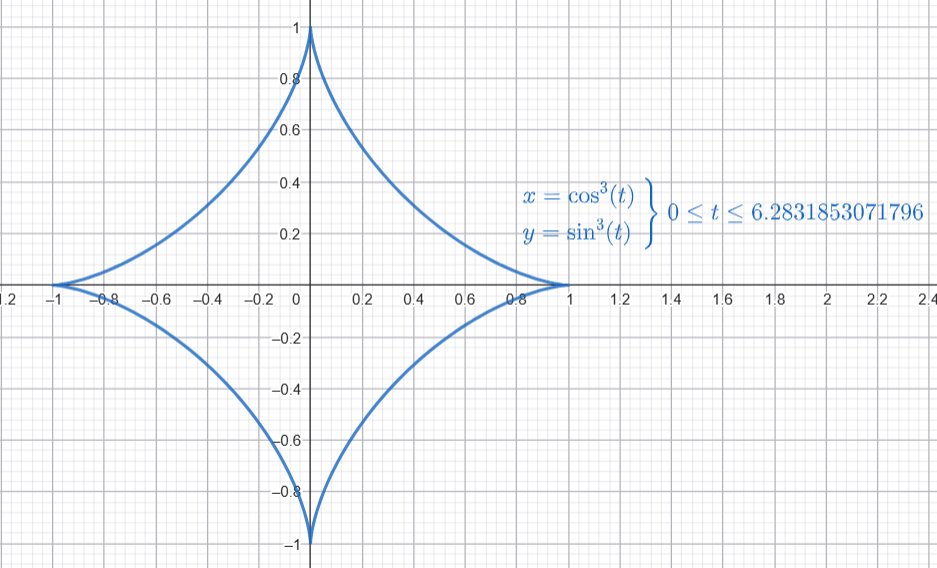
\includegraphics[width=9cm]{5M-2-seda.jusjajeva.INF.png}
\end{figure}

$S = 2\cdot2\pi\integral_0^{\tfrac{\pi}{2}}\left|a\sin^3t\right|\sqrt{((a\cos^3t)')^2+((a\sin^3t)')^2}dt$ \\

$\integral\left|a\sin^3t\right|\sqrt{((a\cos^3t)')^2+((a\sin^3t)')^2}dt$ \\

$= a\integral\sin^3t\sqrt{(-3a\cos^2t\sin t)^2+(3a\sin^2t\cos t)^2}dt$ \\

$= a\integral\sin^3t\sqrt{9a^2\cos^4t\sin^2t + 9a^2\sin^4t\cos^2t}dt$ \\

$= 3a^2\integral\sin^3t\sqrt{\cos^4t\sin^2t + \sin^4t\cos^2t}dt$ \\

$= 3a^2\integral\sin^3t\sqrt{\cos^2t\sin^2t(\cos^2t + \sin^2t)}dt$ \\

$= 3a^2\integral\sin^3t\cos t\sin tdt$ \\

$= 3a^2\integral\sin^4t\cos tdt$ \\

Substitutie: $s = \sin t \Rightarrow ds = \cos tdt$ \\

$= 3a^2\integral s^4ds$ \\

$= \dfrac{3a^2s^5}{5} + c = \dfrac{3a^2\sin^5t}{5} + c$ \\



$\Rightarrow S = 4\pi \left[\dfrac{3a^2\sin^5t}{5}\right]_0^{\tfrac{\pi}{2}} = \dfrac{12a^2\pi\sin^5\dfrac{\pi}{2}}{5}= \dfrac{12a^2\pi}{5}$ \\




\begin{thebibliography}{999}
%\bibitem{a} Referentie
\end{thebibliography}
\end{document}